\documentclass[12pt,a4paper]{article}

\usepackage{amsmath,amssymb,latexsym,amsthm}
\usepackage{enumitem}
\usepackage{multirow}
\usepackage{graphicx}
\usepackage{float}
\usepackage{titlesec}
\usepackage{caption}
\usepackage{subcaption}
\usepackage{biblatex}
\addbibresource{references.bib}
\graphicspath{{Images/}}
\usepackage{hyperref}

\titlespacing\section{0pt}{12pt plus 4pt minus 2pt}{0pt plus 2pt minus 2pt}
\titlespacing\subsection{0pt}{12pt plus 4pt minus 2pt}{-8pt plus 2pt minus 2pt}
\titleformat*{\section}{\large\bfseries}
\titleformat*{\subsection}{\small\bfseries}

\addtolength{\topmargin}{-4\baselineskip}
\addtolength{\textheight}{8\baselineskip}
\addtolength{\textwidth}{2cm}
\addtolength{\oddsidemargin}{-1cm}
\addtolength{\evensidemargin}{-1cm}

\def\nfrac#1#2{{\textstyle\frac{#1}{#2}}}

\newcommand{\nc}{\newcommand}
\def \qedbox{\hfill\vbox{\hrule\hbox{\vrule
height1.3ex\hskip0.8ex\vrule}\hrule}}

\pagestyle{empty}

\setlength{\parskip}{\baselineskip}
\setlength{\parindent}{0mm}

\pagestyle{plain}

\begin{document}


\vspace*{-\baselineskip}

\begin{center}
{\Large {\bf  Modelling Option Values and Stock Price Volatility:\\ A Deep Learning Approach}}
\end{center}

\begin{align*}
    \text{Nam Anh Dang}& \hspace{50pt} \text{z5310809} \\
    \text{Rachel Fitzpatrick}& \hspace{50pt} \text{z5310160} \\
    \text{Purnjay Peshawaria}& \hspace{50pt} \text{z5215940} \\
    \text{Matthew Su}& \hspace{50pt} \text{z5257413} \\
    \text{Rong Tang}& \hspace{50pt} \text{z5276739}
\end{align*}

\section{Introduction}
In the financial world, efficient real-time calculation of option prices is becoming increasingly important. This is done using models that are often multi-dimensional and include nonlinear features. These models often do not have closed form solutions, so numerical methods are used to approximate solutions. However, these methods are often inefficient.

The paper \textit{Pricing options and computing implied volatilities using neural networks} by Liu, Oosterlee and Bohte (\cite{risks7010016}) proposes that Artificial Neural Networks (ANNs) are a viable solution to value options more efficiently. According to the Universal Approximation Theorem, ANNs with one hidden layer and sufficiently many neurons are able to accurately approximate multi-dimensional, non-linear functions. (\cite{risks7010016}) This process involves two phases, the training phase and the prediction phase. While the training phase is slow, it can be completed offline. Once this has been done, the real-time prediction is efficient.

In this paper we will replicate the results of paper \cite{risks7010016}. First we will describe the structure of an ANN and the process of selecting hyper-parameters. We will train two ANNs using data generated by the Black-Scholes option pricing model and the Heston model respectively. Then we will train an ANN to predict implied volatility and compare the accuracy and efficiency of the ANN to Brent's method for approximating implied volatility using the Black-Scholes model.
Additionally, we will extend the work in paper \cite{risks7010016} by comparing the accuracy and run-time performance of ANN on a CPU to the traditional finite difference methods that are currently used by the finance practitioners for option valuation.

\section{The artificial neural network}
\subsection{The structure of an ANN (\cite{risks7010016})}
An artificial neural network (ANN) consists of layers of neurons. The neurons in each layer receive the outputs of the previous layer in order to perform calculations. There is an input layer which receives input from the user, one or more hidden layers and an output layer which returns the results to the user.

As an example, consider a simple multi-layer perceptron with one hidden layer.
\begin{figure}[H]
    \centering
    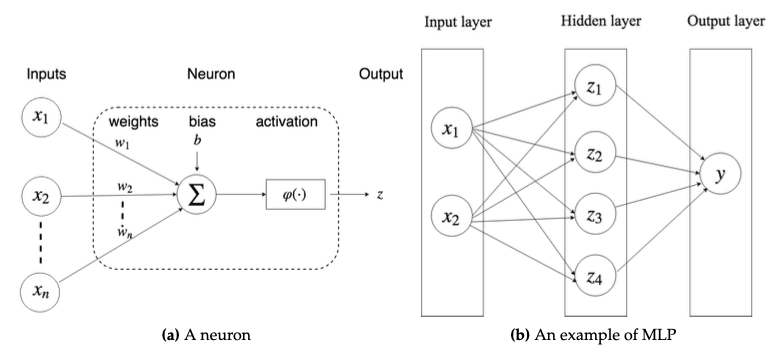
\includegraphics[width=430pt]{neuralNetworkDiagram.png}
    \caption{Structure of a MLP (\cite{risks7010016})}
\end{figure}
Each neuron applies weights to all the inputs and sums them. Then it adds a bias. Finally it applies an activation function to allow for non-linearity. It produces a scalar output that is used as an input for the next layer. If 
\begin{itemize}
    \item $z_j^{(l)}$ is the output of the $j$th neuron in the $l$th layer,
    \item $\phi^{(l)}$ is the activation function,
    \item $w_{ij}^{(l)}$ is the weight of the $i$th input to the $j$th neuron on the $l$th layer, and
    \item $b_j^{(l)}$ is the bias for the $j$ neuron in the $l$th layer,
\end{itemize}
then the output of the neuron is
\begin{align}
    z_j^{(l)} = \phi^{(l)}\left( \sum_i w_{ij}^{(l)}z_i^{(l-1)}+b_j^{(l)} \right).
\end{align}

The whole ANN is defined by the parameters
\begin{align}
    \theta = (\mathbf{W}_1, \mathbf{b}_1, \mathbf{W}_2, \mathbf{b}_2,...,\mathbf{W}_L, \mathbf{b}_L,).
\end{align}

Denote the output of the whole ANN by $F(\mathbf{x} | \theta)$, where $\mathbf{x}$ is the input into the ANN.

\subsection{Hyper-parameter tuning}
We must now make selections for the following hyper-parameters,
\begin{figure}[H]
    \centering
    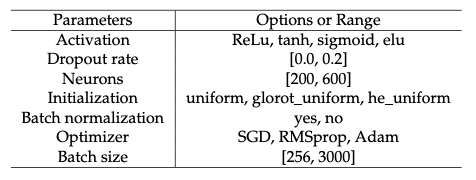
\includegraphics[width=320pt]{hyperparameterRanges.png}
    \caption{Hyper-parameter selection options/ranges (\cite{risks7010016})}
\end{figure}

We use a random search. Generate 1000 data points, divided into an 80\% training set and 20\% validation set. Randomly select 1000 combinations of hyper-parameters from the options in figure 2. For each set of hyper-parameters, train the ANN over 20 epochs, then calculate the MSE on the validation data set. Choose the set of parameters that results in the lowest MSE. In this case the best set of hyper-parameters is shown in the table below, with evaluation loss 6.0146849136799574e-05.

\begin{table}[h!]
\begin{center}
\begin{tabular}{c|c} 
 \hline
 Parameters & Options  \\ [0.5ex] 
 \hline
 Hidden layers & 4   \\ 
 \hline
 Neurons(each layers) & 321  \\
 Activation & elu \\
 Dropout rate & 0.0  \\
 Batch-normalization & no  \\
 Initialization & glorot\_uniform  \\
 Optimizer & Adam  \\
 Batch size & 388  \\ [1ex] 
 \hline
\end{tabular}
\caption{The selected hyper-parameters after the random search.}
\label{table:1}
\end{center}
\end{table}


\subsection{Training the ANN}
The metric of loss function we will use to train the ANN is the mean square error,
\begin{align}
    L(\theta) = MSE = \frac{1}{n}\sum(y_i-\hat{y}_i)^2,
\end{align}
where $y_i$ is the actual value and $\hat{y}_i$ is the output generated by the neural network.
Our goal is to find the values of the weights and biases that minimise the loss function. That is, to find
\begin{align}
    arg\min_\theta L(\theta|(\mathbf{x}, \mathbf{y})).
\end{align}

The parameters are updated using
\begin{align}
    \mathbf{W} \leftarrow \mathbf{W} - \eta(i)\frac{\partial L}{\partial \mathbf{W}}, \nonumber \\
    \mathbf{b} \leftarrow \mathbf{b} - \eta(i)\frac{\partial L}{\partial \mathbf{b}}
\end{align}
for $i=0, 1, 2,...$ representing the iteration number, and $\eta(i)$ the learning rate on the $i$th iteration.

\section{The Black-Scholes option pricing PDE}
The Black-Scholes PDE for valuing European call options is given by
\begin{align}
    \frac{\partial V}{\partial{t}} + \frac{1}{2}\sigma^2S^2\frac{\partial^2V}{\partial S^2}+rS\frac{\partial V}{\partial S} -rV = 0,
\end{align}
with the final condition
    \begin{align}
    V(t=T,S) = (S_0-K)^+,
\end{align}
where
\begin{itemize}
    \item $V(t,S)$ is the option price,
    \item $t$ is the time,
    \item $\sigma$ is the volatility parameter,
    \item $S$ is the price of a non-dividend paying asset at a given time,
    \item $r$ is the risk-free interest rate,
    \item $T$ is the final expiry time,
    \item $S_0$ is the price at maturity, and
    \item K is the strike price of the option.
\end{itemize}

A solution to (6) and (7) for European plain vanilla options is given by
\begin{align}
    V_c(t,S) &= SN(d_1) - Ke^{-r\tau}N(d_2), \nonumber \\
    d_1 &= \frac{\text{log}(\frac{S}{K}) + (r + 0.5\sigma^2)\tau}{\sigma\sqrt{\tau}}, \\
    d_2 &= d_1 - \sigma\sqrt{\tau}, \nonumber
\end{align}
where $V_c$ is the European call option value, $\tau := T-t$ and $N(\cdot)$ is the normal distribution. We will denote this solution by $V(\cdot)=BS(\cdot)$.

\subsection{Generating the data set using the Black-Scholes model}
Generate 1,000,000 samples of the input parameters of the Black-Scholes model within the ranges defined in figure 3. Use the closed form solution to the Black-Scholes model in equation $(8)$ to calculate the scaled option price, $V$. To generate examples, the table below was used alongside a uniform distribution for each parameter. Both wide range and narrow range was used to generate the data.

\begin{figure}[H]
    \centering
    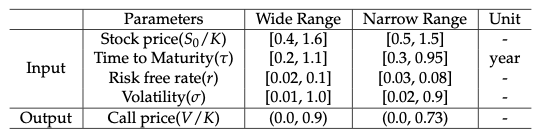
\includegraphics[width=370pt]{Black-Scholes parameter ranges.png}
    \caption{Black-Scholes parameter ranges (\cite{risks7010016})}
\end{figure}

\subsection{Training the ANN and selecting the learning rate}
Initially, training the ANN was tested using the wide range column and non-tuned hyper parameters. The hyper-parameters used were a learning rate of 0.001, 200 epochs, RELU activation, 0 dropout rate, 400 hidden layer neurons, glorot uniform, non batch-normalization and Adam optimization. The results for each epoch had constant training and validation loss at around 0.105.
We decided to use a package called torch-lr-finder to find the best learning rate in order to improve the training of the model. After testing 100 different learning rates within the interval [0.00001 to 0.001], the best learning rate had the steepest gradient.
\begin{figure}[H]
    \centering
    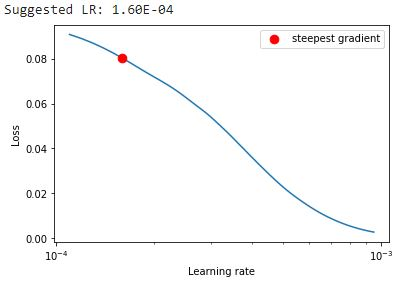
\includegraphics[scale=1]{Best learning rate for ANN for wide range.JPG}
    \caption{Best learning rate for training the ANN}
\end{figure}
After inputting $1.60 \cdot 10^{-4}$ as the learning rate to our ANN, the training of the model significantly improved. The graph below shows the improvement of the MSE loss.
\begin{figure}[H]
    \centering
    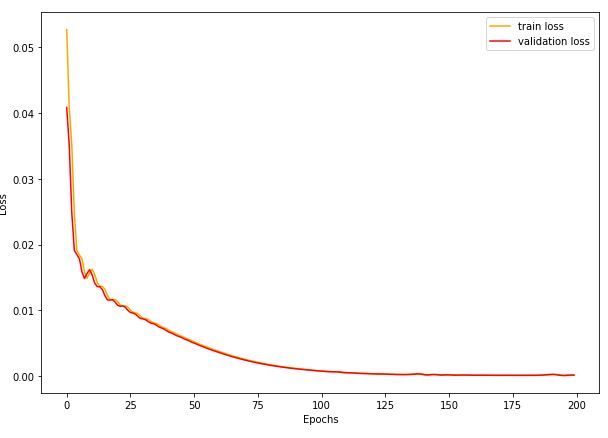
\includegraphics[scale=0.8]{ANN Option Pricing MSE loss.JPG}
    \caption{Training the ANN model on the new learning rate}
\end{figure}
The final MSE loss for the training and validation set was $1.89 \cdot 10^{-4}$ and $1.66 \cdot 10^{-4}$ respectively.\\\\
Next, the hyper parameters from section (2.2) was used and trained with the ANN model. The results were a huge improvement from the previous training.
\begin{figure}[H]
    \centering
    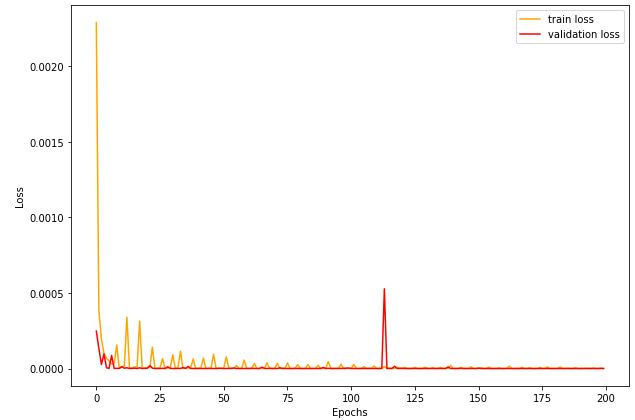
\includegraphics[scale=0.8]{Best learning rate and tuned hyperparameter for ANN for wide range.JPG}
    \caption{Training the ANN model after tuning hyperparameters}
\end{figure}
Particularly, the MSE loss for the training and validation set was $1.18\cdot 10^{-8}$ and $2.06 \cdot 10^{-8}$ respectively. This result nearly matched the MSE loss in the paper at $8.04 \cdot 10^{-9}$. Due to time constraints and GPU constraints on Google Colab, we were not able to train the model on the narrow range.

\section{The Heston Model}
One of the flaws of the Black-Scholes model is that it assumes a constant volatility. However financial data indicates that volatility is variable (\cite{risks7010016}). A class of models called stochastic volatility (SV) models account for this by treating the volatility as a random variable. These models more accurately represent the smile or skew volatility shapes in the real life market data, especially for options with a long time to the maturity date.

The Heston model is a commonly used SV model. It is represented by the following system of SDEs,
\begin{align}
    &dS_t = rS_tdt + \sqrt{v_t}S_tdW_t^s, \hspace{15pt} S_{t_0}=S_0, \nonumber \\
    &dv_t = \kappa(\bar{v}-v_t)dt + \gamma\sqrt{v_t}dW_t^v, \hspace{15pt} v_{t_0}=v_0, \\
    &dW_t^sdW_t^v = \rho dt, \nonumber
\end{align}
where
\begin{itemize}
    \item $S_t$ is the asset price at time $t$,
    \item $r$ is the risk-free interest rate,
    \item $v_t$ is the instantaneous variance,
    \item $\kappa$ is the reversion speed,
    \item $\bar{v}$ is the long term variance,
    \item $\gamma$ is the volatility of the variance, and
    \item $\rho $ is the correlation coefficient of the Weiner processes $W_t^s, W_t^v$.
\end{itemize}

From this we can derive the following Heston option pricing PDE,
\begin{align}
    \frac{\partial V}{\partial t} + rS\frac{\partial V}{\partial S} + \kappa(\bar{v}-v)\frac{\partial V}{\partial v} + \frac{1}{2}vS^2\frac{\partial^2V}{\partial S^2} + \rho\gamma Sv\frac{\partial^2V}{\partial S\partial v} + \frac{1}{2}\gamma^2v\frac{\partial^2 V}{\partial v^2} -rV = 0.
\end{align}

This PDE does not have a closed form solution, so the option value is determined using the COS method, which approximates the probability density function of the asset price using Fourier-cosine series expansions. 

\subsection{The COS method}

The COS method was first described by Fang, F. \& Oosterlee, K. (2008) (\cite{hestonfo}). As for the values of $a$ and $b$, we use the procedure below which is derived from Fitt et al. (2010) (\cite{fitt_wilson_ockendon_norbury_2010}). We first denote $k$ as the indices in range $1,2,\dots,N$ of $N$ terms of a Fourier-cosine series, and $[a, b]$ as the integration interval for the series.

We first need the cosine series coefficients of $g(y)=e^y$ and $g(y)=1$ on the interval $[c, d] \subset [a, b]$, denoted as $\chi_k$ and $\psi_k$ respectively:
\begin{align}
    \nonumber
    \chi_k(c, d) = \frac{1}{1+\left(\frac{k\pi}{b-a}\right)^2} \Biggl[ \cos\left(k\pi\frac{d-a}{b-a}\right)e^d - \cos\left(k\pi\frac{c-a}{b-a}\right)e^c + 
\\
\frac{k\pi}{b-a}\sin\left(k\pi\frac{d-a}{b-a}\right)e^d -  \frac{k\pi}{b-a}\sin\left(k\pi\frac{c-a}{b-a}\right)e^c \Biggr],
\end{align}
\begin{align}
\psi_k(c, d) = \begin{cases}
      \left[\sin\left(k\pi\frac{d-a}{b-a}\right) - \sin\left(k\pi\frac{c-a}{b-a}\right)\right]\frac{b-a}{k\pi} & k \neq 0\\
      (d-c) & k=0.
    \end{cases} 
\end{align}

Next, we find the call and put \textit{payoff series coefficients}, $U_k$:
\begin{align}
    U_k^{call} &= \frac{2}{b-a}K(\chi_k(0,b)-\psi_k(0,b)),\\
    U_k^{put} &= \frac{2}{b-a}K(\psi_k(a,0)-\chi_k(a,0)).
\end{align}

Letting $\phi_k$ be the value of the characteristic function of the PDE evaluated at the values of $k$, then the call option value $V_k$ can be approximated as follows:
\begin{align}
    \nonumber
    I_k &= \exp\left(ik\pi \frac{x-a}{b-a}\right)\\
    \nonumber
    F_k &= \text{Re}\left( \phi_k \odot I_k \right)\\
    \nonumber
    F_{k1} &= \frac{1}{2} \cdot F_{k1}\\
    V_k^{call} &= K \left[\sum_{i=1}^{N} F_k \odot U_k^{call}\right] \cdot \exp(-r\tau)\\
    V_k^{put} &= K \left[\sum_{i=1}^{N} F_k \odot U_k^{put}\right] \cdot \exp(-r\tau),
\end{align}
where $\odot$ denotes pointwise multiplication of vectors of size $N$ and $F_{k1}$ denotes the first element of $F_k$.

An equivalent value of $V_k^{call}$ can be found using the relationship of the put-call parity:
\begin{align}
    V_k^{call} = V_k^{put} + S - K\exp(-r\tau).
\end{align}

To use the COS method to approximate the call prices using the Heston model, we need the value of the characteristic function $\phi_k$ of the Heston PDE:
\begin{align}
    \nonumber
    \phi_k &= \exp\Bigg( iur\tau + \frac{v_0}{\gamma^2} \Bigg( \frac{1-\exp(-D\tau)}{1-G\exp(-D\tau)} \Bigg) (\kappa-i\rho\gamma u )\Bigg)\\
    &+ \exp\Bigg( \frac{k\bar{v}}{\gamma^2}\Bigg( \tau(\kappa-i\rho\gamma u)-D)-2\log\Bigg( \frac{1-G\exp(-D\tau)}{1-G} \Bigg) \Bigg) \Bigg),
\end{align}
where
\begin{align*}
u &= \frac{\pi}{b-a} \cdot k,\\
D &= \sqrt{(\kappa-i\rho\gamma u)^2+(u^2+iu)\gamma^2},\\
G &= \frac{\kappa-i\rho\gamma u-D}{\kappa-i\rho\gamma u+D}.
\end{align*}

As for the values of $a$ and $b$, we use the procedure below which is derived from Fitt et al. (2010) (\cite{fitt_wilson_ockendon_norbury_2010}), which depends on a single parameter $L$:
\begin{align*}
    c_1 &= r \tau + \frac{(1+\exp(-\kappa\tau)\cdot(\bar{v}-v_0)}{2\kappa} - \frac{\bar{v}\tau}{2}\\
    c_2 &= \frac{\gamma\tau\kappa\exp(-\kappa\tau)\cdot(v_0-\bar{v})\cdot(8\kappa\rho-4\gamma)}{8\kappa^3}\\
    &+ \kappa\rho\gamma\cdot(1-exp(-\kappa\tau))\cdot(16\bar{v}-8v_0)\\
    &+ 2\bar{v}\kappa\tau\cdot(-4\kappa\rho\gamma+\gamma^2+4\kappa^2)\\
    &+ \gamma^2\cdot((\bar{v}-2 v_0)\cdot\exp(-2\kappa\tau) + \bar{v} \cdot(6\exp(-\kappa\tau)-7) + 2 v_0)\\
    &+ 8\kappa^2\cdot(v_0-\bar{v})\cdot(1-\exp(-\kappa\tau))
\end{align*}
\begin{align}
    a = c_1 - L\sqrt{\lvert c2 \rvert}\\
    b = c_1 + L\sqrt{\lvert c2 \rvert}.
\end{align}

\subsection{Training the ANN}

For the target $V$, we generated 1,000,000 samples of European call prices using the COS method for the Heston model, with the input parameters within the ranges defined in Figure 7. When $S < K$, we used the put-call parity since the call value from the COS method can be inaccurate. 

\begin{figure}[H]
    \centering
    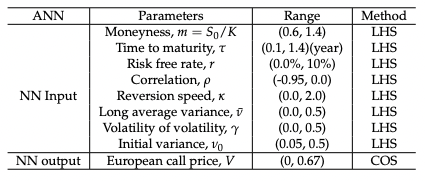
\includegraphics[width=310pt]{hestonParameterRanges.png}
    \caption{Heston parameter ranges}
\end{figure} 

From Figure 7, the expected range of the output $V$ is $(0, 0.67)$. While most of the values generated were in this range, there were some inaccuracies on both ends of the range. To fix this, an option price by definition cannot be negative, so we changed any negative values to 0. However, to avoid extra tampering with the target data, we do not cap any values that are over 0.67 down to 0.67.

For the other parameters, we set a fixed strike price of $K=1$, $L=50$ to compute $a$ and $b$ and $N=1500$ terms in the Fourier-cosine series.

We trained an ANN with the inputs being the 8 parameters in Figure 7, with 400 neurons in each hidden layer and a learning of 0.001, the upper range used in the paper, and MSE for the optimizer. While the original paper used 3000 epochs, we used 1000 epochs due to runtime constraints.

\begin{figure}[H]
    \centering
    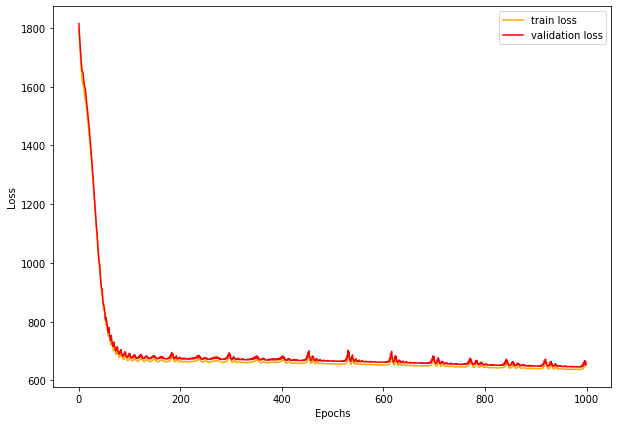
\includegraphics[width=370pt]{hestonLossGraph.png}
    \caption{Training and validation losses of the Heston ANN}
\end{figure}

As we can see from Figure 8, both the training and validation loss converges to around 625. One possible reason that the loss does not go down to 0 is that our target values still have some outliers that are greater than 0.67, which are out of the expected range. More focus on finding suitable values $a$ and $b$ for the integration range could allow for a more accurate approximation of the target values, which could lower the loss that the model will converge to. 

Furthermore, the loss already converges to around the minimum epoch of 625 after 200-300 epochs, so there is likely not much difference from training for 1000 epochs compared to 3000 epochs.

\section{Predicting implied volatility}
Next we will train an ANN to predict implied volatility based on option price. We will also predict implied volatilities using Brent's method and demonstrate that the ANN performs the prediction more quickly.

\subsection{Training the ANN}
The data to train the ANN was generated as follows. Generate 1,000,000 values for the risk free rate $r$, the volatility $\sigma$, the time to maturity $\tau$ and the scaled stock price $\frac{S}{K}$ according to a uniform distribution within the ranges in the table below.

\begin{figure}[H]
    \centering
    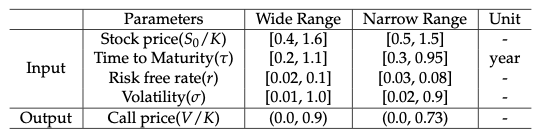
\includegraphics[width=370pt]{Black-Scholes parameter ranges.png}
    \caption{Parameter ranges for training ANN to predict implied volatility (\cite{risks7010016})}
\end{figure}

Calculate the target option values $V$ using the Black-Scholes model.

The option Vega is the derivative of the option price with respect to the implied volatility. The option Vega may be very small, in which case the derivative of implied volatility with respect to option price is large. When the gradient is large, the prediction error of an ANN may be large. The paper \cite{risks7010016} uses a gradient-squash method to mitigate this issue. Set
\[ \bar{V} = V_t - \text{max}(S_t-Ke^{-r\tau}, 0). \]

Scale the option value by $\frac{1}{K}$ then apply a log transform to produce the scaled time value log$\left(\frac{\bar{V}}{K}\right)$. Since the log of 0 is undefined, remove all data points with $\bar{V} < 10^{-7}$.

Train the ANN over 200 epochs with the hyper-parameters selected in section 2.2 to predict $\sigma$ given the stock price, time to maturity, risk-free rate and scaled time value as input. The MSE loss for each epoch is depicted in Figure 10.

\begin{figure}[H]
    \centering
    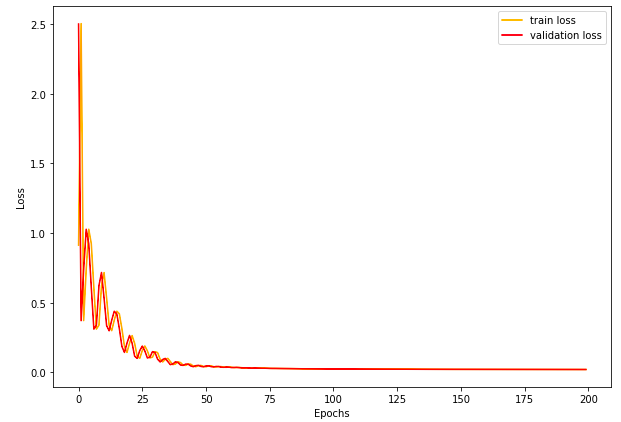
\includegraphics[width=450pt]{impliedVolatilityANNTrainingGraph.png}
    \caption{Loss per epoch during training}
\end{figure}

\subsection{Brent's method}
Denote the implied volatility by $\sigma^*$ and an observed market option price as $V^{mkt}$. The implied volatility is calculated using the Black-Scholes model by solving
\[ BS(\sigma^*; S,K,\tau,r)=V^{mkt}. \]
We cannot find an analytic solution for $\sigma^*$. Instead we write
\begin{align}
    g(\sigma^*) = BS(S,\tau,K,r,\sigma^*)-V^{mkt}(S,\tau;K) = 0
\end{align}
and use a numerical iterative technique to find the roots of $g$.

A possible numerical method to find the zeros of $g$ is Brent's method. At each iteration Brent's method uses the update
\begin{align}
    \sigma_{k+1} &= \frac{\sigma_kg(\sigma_{k-1})g(\sigma_{k-2})}{(g(\sigma_{k})-g(\sigma_{k-1}))(g(\sigma_k)-g(\sigma_{k-2}))} \nonumber \\
    &+ \frac{\sigma_{k-1}g(\sigma_{k-2})g(\sigma_{k})}{(g(\sigma_{k-1})-g(\sigma_{k-2}))(g(\sigma_{k-1})-g(\sigma_{k}))} \\
    &+ \frac{\sigma_{k-2}g(\sigma_{k-1})g(\sigma_{k})}{(g(\sigma_{k-2})-g(\sigma_{k-1}))(g(\sigma_{k-2})-g(\sigma_{k}))}, \nonumber
\end{align}
where $\sigma_{k-2}$, $\sigma_{k-1}$ and $\sigma_{k}$ are the three previous iterants. When two consecutive points are the same, we instead use the update
\begin{align}
    \sigma_{k+1} = \sigma_{k-1} - g(\sigma_{k-1})\frac{\sigma_{k-1} - \sigma_{k-2}}{g(\sigma_{k-1})-g(\sigma_{k-2})}.
\end{align}

\subsection{Comparison of the ANN and Brent's method for predicting implied volatility}
Generate 20,000 true $\sigma$ values in the range [0.011, 0.99]. For all data points set the risk-free rate $r=0$, the time to maturity $\tau=0.5$, $K = 1$, and $S = 1$. Calculate the market values using the Black-Scholes model.

Apply the gradient-squashing and log transform method described above to the data that will be used by the ANN.

Use the trained ANN and Brent's method with a tolerance of 0.0001 to predict the implied volatilities. The MSE and CPU time for each is recorded in the following table.

\begin{center}
\begin{tabular}{ |c|c|c| } 
 \hline
 Method & MSE & CPU time (sec) \\ 
 \hline
 Brent's Method & 0.0383 & 30.3267 \\ 
 ANN & 0.0574 & 0.3106 \\ 
 \hline
\end{tabular}
\end{center}

It is clear that prediction using the ANN is considerably faster than prediction using Brent's method.

\section{Finite Difference Methods for Valuation of Options}
The idea behind using finite differences to value options is that under a suitable transformation and change of variable, the Black-Scholes PDE can be converted into the heat equation and there are many finite difference methods to solve this equation. We convert the Black-Scholes PDE into a difference equation by discretising the time variable and stock-price in the following manner:

We choose a uniform step-size $\Delta t$ such that $t_n = n\Delta t$ where $n$ (the number of data points) ranges from $0$ to $N_t$ where $N_t$ is the total number of sub-intervals. Note that $0 \leq t_n \leq T \,\,\forall n.$ Here T is the final expiry time of the option. Similarly, we discretise $S$ such that $S_j = j\Delta S$ where the number of instances, $j$, ranges from $0$ to $N_s.$ Here, $N_s$ is the total number of sub-intervals for discretising $S.$ Also $S_j$ ranges from $0$ to $S_{max} \,\,\forall j$. Consequently, we get the following discrete boundary conditions
\begin{align*}
    V_0^n &= 0 \text { for } 0 \leq n \leq N_t,\\
    V_{N_s}^n &= S_{\max} - K e^{-r(T - t_n)} \text { for } 0 \leq n \leq N_t,
\end{align*}
and the discrete initial condition
\[
V_j^{N_t} = (S_j - K)^{+} \text { for } 1 \leq j \leq N_s - 1.
\]

There are broadly three finite difference methods: Explicit-Euler, Implicit-Euler and Crank-Nicolson method. The explicit finite difference scheme uses backward difference approximation for $\frac{\partial V}{\partial t}$ and is conditionally stable i.e. it is only stable when the ratio $\frac{\Delta t}{\Delta S^2}$ is below a certain threshold. On the other hand, implicit scheme approximates $\frac{\partial V}{\partial t}$ using a forward difference and is unconditionally stable. The Crank-Nicolson method averages the implicit and explicit schemes. It is unconditionally stable and achieves $\mathcal{O}(\Delta t^2 + \Delta S^2)$ accuracy compared to $\mathcal{O}(\Delta t + \Delta S^2)$ for both the implicit and explicit method. Since the theme of the paper is Machine Learning and Deep Learning, we will not go into the basics of deriving these methods or laying the groundwork for all the necessary equations. The reader is encouraged to read (\cite{intHoutKarel2017NPDE}, \cite{HighamDesmondJ.2004}, ) for additional information about the use of finite difference methods in financial mathematics and basics of numerical analysis.

\subsection{Comparison between FDM and ANN}

Our simulation results are based on the following values:
$K= \$1$, $r \in [0.02, 0.1]$, $\sigma \in [0.01, 1.0]$, $T = 1.1$ years, and 1000 samples for $S$ ranging from $0$ to $S_{max} = 1.6K.$ We computed the European call option value at $t= 0.$ In other words, $\tau = T= 1.1.$

\begin{figure}[H]
\begin{subfigure}{0.5\textwidth}
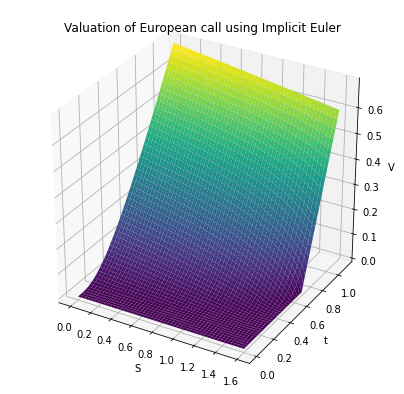
\includegraphics[width=0.9\linewidth, height=5cm]{implicit_FDM_option_value.png} 
\caption{Valuation of call option using Implicit FDM}
\label{fig:subim1 implicit sol}
\end{subfigure}
\begin{subfigure}{0.5\textwidth}
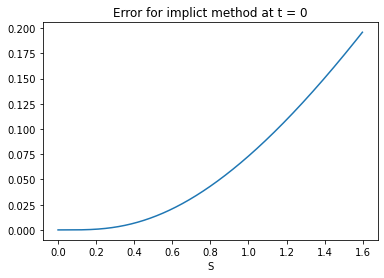
\includegraphics[width=0.9\linewidth, height=5cm]{implicit_FDM_error.png}
\caption{Error for implicit method at $t = 0$}
\label{fig:subim2 implicit err}
\end{subfigure}

\caption{Implicit Euler FDM}
\label{fig:implicit scheme}
\end{figure}

\begin{figure}[H]
\begin{subfigure}{0.5\textwidth}
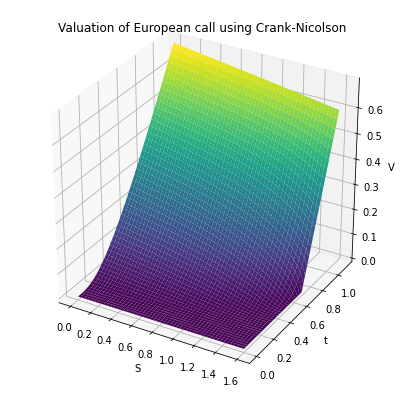
\includegraphics[width=0.9\linewidth, height=5cm]{CN_option_value.png} 
\caption{Valuation of call option using Crank-Nicolson method}
\label{fig:subim1 CN sol}
\end{subfigure}
\begin{subfigure}{0.5\textwidth}
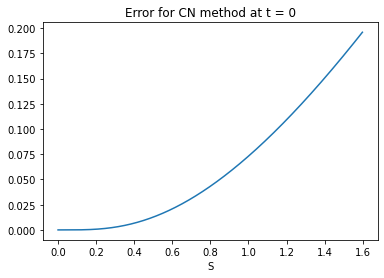
\includegraphics[width=0.9\linewidth, height=5cm]{CN_error.png}
\caption{Error for CN method at $t = 0$}
\label{fig:subim2 CN err}
\end{subfigure}

\caption{Crank-Nicolson FDM}
\label{fig:CN scheme}
\end{figure}
We now compare the results of finite difference methods with ANN.
The MSE and CPU time for each is recorded in the following table.

\begin{center}
\begin{tabular}{ |c|c|c| } 
 \hline
 Method & MSE & CPU time (sec) \\ 
 \hline
 Implicit FDM & 0.007483 & 49.2964 \\ 
 Crank-Nicolson FDM & 0.007480 & 50.2515 \\
 ANN & 0.000721 & 5.12418 \\ 
 \hline
\end{tabular}
\end{center}

It is clear that option value computation using the ANN is considerably faster and more accurate than computation using FDM methods. Note that because of the numerical
instability of the explicit scheme, we did not get any sensible results and thus, we do
not report any MSE for it.

\section{Summary and Future Work}
As highlighted by our research, there is massive scope for using deep learning algorithms in the financial markets. They give superior results both in terms of speed and accuracy to the traditional numerical methods that are currently used by finance practitioners and industry quants. We would like to explore this direction in the future. However, our paper does not eschew use of numerical methods. As noted in this paper (\cite{JANG202143}), real market call option data are imbalanced data consisting mostly of In the Money (ITM) options whereas real market put option data are mostly comprised of Out of the Money (OTM) options. This can make it extremely difficult for the ANN to learn the weights of the input parameters correctly. The authors propose a combination of parametric methods, namely Black-Scholes model, FDM, binomial-option pricing methods, Monte-Carlo simulations to generate additional distilled balanced training data to solve the imbalance problem and therefore, improve the accuracy of ANN. 

\printbibliography

\end{document} 